\section{Macro implications of perceived job risks}

\subsection{Shocks or risks?}

In the previous sections, with the three measures in hand, namely (a) perceived risks, $\widehat{JF}$/$\widetilde{JS}$, (b) objective risks $\widehat{JF}^*$/$\widehat {JS}^*$, and (c) realization of job flow rates $JF$/$JS$, we have established two major findings. The first is a rejection of perfect foresight, in that even ex-ante rational and fully informed forecasts of risks don't fully predict ex-post realizations.  This is indicated by the gap between (b) and (c). The second is the deviation of ex-ante perceived job risks from its true ex-ante counterpart, at least partially due to information rigidity.  

But do the distinctions between (a), (b), and (c) matter for aggregate fluctuations? We can assess empirically the relative importance of ex-ante precautionary saving motives resulting from perceived job risks (a), responses due to misperceived risk ((a)- (b)), and ex-post responses due to truly unexpected income shocks ((b)-(c)), by comparing the cyclical properties of (a), (b) and (c) across business cycles. 

We use two sets of metrics to evaluate the relative importance of the three channels. The first one is the unconditional standard deviation of (a), (b), and (c). The second metric is the ratio between the onset and the end of each recession in our sample. More intuitively, they reflect the changes in these rates from the peak to the trough of each cycle. 

Throughout our data sample 1990-2024 which covered four recessions and experienced sizable cyclical movements of unemployment risks, the unconditional standard deviation of realized job-finding rates is approximately 7.2 percentage points. Most of these variations are reflected in real-time finding probabilities, whose standard deviation was about 6.9 percentage points. In contrast to these cyclical movements of realized job finding rates, the perceived finding rates exhibit milder fluctuations and have a standard deviation of 4 percentage points. In the domain of job separation, the unconditional standard deviations of perceptions, risk forecast, and realizations are 1.0, 0.9, and 0.3 percentage points, respectively. Both finding and separation perceptions move significantly less than the realized job risks. 

Such rankings of the relative volatility of perceptions and realizations also can be seen in Figure \ref{fig:bus_cycle_stats} which reports the peak and trough rates in each of the four recessions in the sample period. From the onset of each recession to its end month, the real-time job finding drops by 25\%, while the perceptions of job finding only decrease by 15\%. 

Meanwhile, average job separation perceptions are much more sluggish than job finding expectations, which is again confirmed by on average a 16\% increase from the start to the end of each recession, as opposed to a 50\% average increase in job separation risk forecast and 150\% in realized job separation rates. The increase in realized job separation rates remains high with the pandemic recession excluded, which was not reflected in the change in perceptions.  

\begin{figure}[pt] 
\centering 
	\caption{Business Cycle Patterns of Risks and Perceptions: Start versus End of Recessions} 
	\label{fig:bus_cycle_stats}
\includegraphics[width=0.99\linewidth]{text/chapter2/Figures/business_cycle_JF_peak_trough.pdf} \\
\includegraphics[width=0.99\linewidth]{text/chapter2/Figures/business_cycle_JS_peak_trough.pdf} \\
 	
    	\begin{flushleft}\footnotesize {Note: The left tables report the perceived job risks, perceived job risks at different quantiles, real-time job risks, and realized job transition rates at the beginning and the end month of each one of the four recessions. The bar chart on the right plots the peak-to-trough ratios of these rates. The sample period is 1990-2024.} \end{flushleft}
\end{figure}

Such average patterns mask substantial heterogeneity in job risks and perceptions. Figure \ref{fig:bus_cycle_stats} also plots the movements of perceptions over business cycles by agents at different percentiles of perceived job risks. In terms of job-finding, although an average worker's perceived job finding probability drops by 15\% from the peak to trough of a recession, more or less comparable to the realized job finding, it is the low-finding rate worker, at 25 percentile who perceive a much sharper drop by about 25\%, compared to a drop of 10\% for the worker at the 75th percentile. In terms of job separation, although an average worker's job loss perceptions only increase by 15 percentage points in recessions, the \emph{median} worker's perceptions increased much more sharply by about 35 percentage points. Recessions hit agents in the economy unevenly in terms of their job risks. Such heterogeneity in perceptions reveals the uneven footprints of business cycle fluctuations via job risk changes. Heterogeneity in risk exposure implies different degrees of ex-ante precautionary saving behaviors and their consequent ex-post shock responses, a topic we turn to in the next section. 


%Using perceived risk and realized flow rates, we can also construct true unexpected shocks to job risks in business cycles and see their effects on consumption spending. 

%Our estimated heterogeneity in job risks the distribution of $\eta_{i,t}$ and the average information rigidity $\lambda$ for each group can be used to calibrate HANK models featuring belief distortions and heterogeneous job risks.

\subsection{Quantifying the aggregate consumption impacts of unemployment risks}

Despite its debatable quantitative importance, an expanding literature has demonstrated that counter-cyclical unemployment risk is an important mechanism that amplifies business cycle fluctuations.\footnote{\cite{challe2016precautionary}, \cite{mckay2017time}, \cite{bayer2019precautionary}, \cite{ravn2021macroeconomic}.} Almost all of these models, however, assume perfect foresight and full-information-rational expectations. That is, (a), (b), and (c) are assumed to be the same object.\footnote{\cite{bardoczy2023unemployment} is an exception, which incorporates deviation in perceived job risks in an otherwise standard HANK model.} Unlike them, we pay special attention to implications of the fact that it is subjectively perceived job risks, as we measured separately, that effectively govern ex-ante precautionary saving behaviors. We show in this section that the quantitative importance of the unemployment risk channel crucially depends on how such risks are perceived by the households. 

\subsubsection*{Decomposition of consumption Jacobians}

 The overall impacts of unemployment risks on consumption not only depend on how big the fluctuation of the actual and perceived risks is, which is the primary focus of the paper but also the sensitivity of the aggregate consumption response to changes in unemployment risks. We discipline such sensitivity with a heterogeneous-agent consumption-saving model featuring persistent unemployment under a set of standard calibrations commonly seen in the literature. In our model, households make a consumption-saving decision in the face of both productivity shocks and unemployment risk. Unemployment risk is dictated by the job separation and job finding probability. Self-insurance is achieved by saving money on a risk-free bond. Figure \ref{fig:model_timeline} illustrates the timeline of the model and we document other model specifications in the Appendix \ref{appendix:model}. Table \ref{table:Calibration} reports all the parameter calibrations. What's particularly important is the unemployment insurance replacement ratio, which we set to be 0.5. We indirectly infer the discount factor $\beta$ to be 0.97 to match a steady state quarterly MPC of 0.16, which falls well in the median range of the estimates seen in the literature. The model is set at a quarterly frequency. \ footnote \footnote{In the Appendix, we reproduce our experiments with a monthly model with several modifications. The main messengers to be conveyed in the following discussions remain intact.} 


\begin{figure}[pt]
    \centering
    \caption{Timeline of the Model}
    \label{fig:model_timeline}
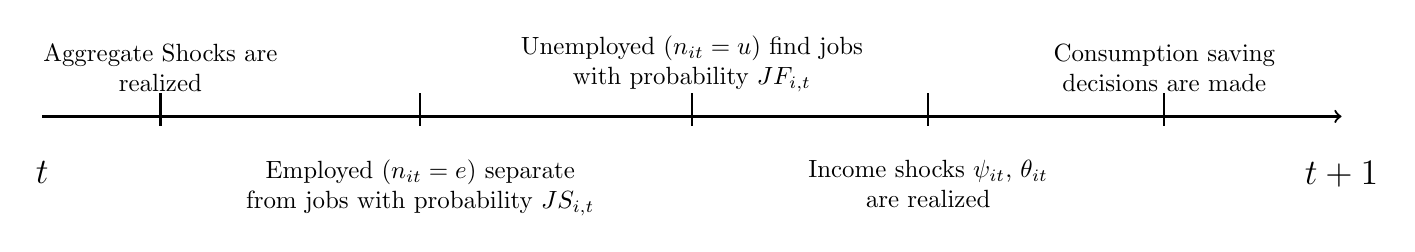
\begin{tikzpicture}[thick,scale=1.5, every node/.style={scale=.9}]
  % Set the timeline's limits
  \draw[->] (0,0) -- (11,0);
  \draw (11,-.3) node[below] {\Large $t+1$};
  \draw (0,-.3) node[below] {\Large $t$};
  % Add events
  \draw (1.,-.08) node[above=10pt,align=center] {Aggregate Shocks are\\realized} -- (1.,0.2);
  \draw (3.2,-.08) node[below=10pt,align=center] {Employed ($n_{it}=e$) separate\\from jobs with probability $JS_{i,t}$} -- (3.2,.2);
  \draw (5.5,-.08) node[above=10pt,align=center] {Unemployed ($n_{it}=u$)  find jobs\\with probability $JF_{i,t}$} -- (5.5,0.2);
  \draw (7.5,-.08) node[below=10pt,align=center] {Income shocks $\psi_{it}$, $\theta_{it}$ \\are realized} -- (7.5,0.2);
  \draw (9.5,-.08) node[above=10pt,align=center] {Consumption saving\\decisions are made} -- (9.5,0.2);

\end{tikzpicture}
\end{figure}

 %that the dynamic response of aggregate consumption to job risks can be characterized by multiplying the time paths of the job risks and the Jacobians that measure the elasticity of total consumption toward per unit change in job risks at future different horizons. %The empirical size of the changes in job risk perceptions and realizations are obtained from our empirical measures (a), (b), and (c). The Jacobians come from solving the heterogeneous-agent model's forward-looking optimization problem given the anticipated shock and obtaining aggregate responses relative to its steady state resulting from the change in consumption policies and realized income shocks.
 
In the model, the dynamic aggregate consumption response comes from both the optimally chosen consumption policies of heterogeneous households given their perceived risks and the resulting changes in the wealth distribution, which come from both choices and the realized unemployment shocks. We summarize such responses using the Sequence Space Jacobian method by \cite{auclert2021using}. 

As an illustration, the consumption Jacobians concerning a future positive shock to job separation rate at a given horizon are shown in Figure \ref{fig:jac_decompose} under the standard perfect foresight assumption, in that the shock to future job risks at $t+h$ ($h$=10 here) is perfectly anticipated by agents at the time $t$. The ex-ante component Jacobians include both the consumption response between $t$ and $t+h$ and the subsequent impacts of such self-insurance behaviors on the consumption response after the shock realization. The ex-post Jacobians capture the consumption impacts in effect from $t+h$ when the shock happens. It is calculated by fixing the consumption policy of the agents but unexpectedly increasing the job risks at $t+h$. Essentially, it measures the aggregate consumption impacts of a higher share of people who unexpectedly find or lose their jobs. The total Jacobians consist of both the ex-ante and ex-post responses. Intuitively, because of the ex-ante responses before the realization of the shock, the hypothetical ex-post responses to the realized shock at $t+h$ are partially insured, resulting in a more moderate total response at the moment of the shock.  

\begin{figure}[pt]
    \centering
    \caption{Consumption Jacobian to an anticipated 10-period-ahead shock to the job separation}
    \label{fig:jac_decompose}
%\includegraphics[width=0.9\textwidth]{Figures/JF_decomposition.pdf} 
\includegraphics[width=0.8\textwidth]{text/chapter2/Figures/JS_decomposition.pdf} 
\floatfoot{\footnotesize{This figure plots the total and decomposed Jacobians of the aggregate consumption with respect to an anticipated shock to job separation probability at $t+10$. The Jacobian is defined exactly as in \cite{auclert2021using}. }}
\end{figure}

With the same logic, we can decompose the aggregate consumption Jacobians into ex-ante and ex-post responses under subjective perceptions of job risks, as shown in Figure \ref{fig:jac_decompose_sub}. The total response with belief rigidity differs from its objective benchmark, which ultimately comes from a different ex-ante response. In particular, the ex-ante subjective response is entirely based on how the imagined shock at $t+h$ is perceived by the agent at time $t$. Because of belief stickiness, subjective ex-ante Jacobian jumps downward less than the full-information one. This also results in a more drastic drop in consumption following the shock at $t+h$ than in the full-information case (``Subjective (Total)"), simply because the consumption insurance induced by ex-ante response was more limited (``Subjective ex-ante") to counteract the impacts of uninsured ex-post shock (``ex-post").


What is more interesting is that we can understand the difference between the objective and subjective perceptions of job risks through the lens of ex-ante/ex-post decomposition. In particular, the total subjective responses (``Subjective (Total)") can be further thought of as a combination of the contributions from the ex-ante response under sticky expectations (``Subjective ex-ante"), underinsurance due to misperceived risks due to stickiness (the area between ``Subjective ex-ante" and "Objective ex-ante"), and the responses under full-information (``Objective (Total)"). Due to the under-insurance toward the increased job separation risk, the consumption drop following the shock is bigger than that under full information.  


\begin{figure}[pt]
    \centering
    \caption{Subjective Consumption Jacobians with Sticky Expectations}
    \label{fig:jac_decompose_sub}
%\includegraphics[width=0.8\textwidth]{Figures/JF_decomposition_subjective.pdf} \\
\includegraphics[width=0.8\textwidth]{text/chapter2/Figures/JS_decomposition_subjective.pdf} 
\begin{flushleft}\footnotesize {Note: The figure shows the aggregate consumption Jacobian concerning a future shock to job-separation rate that is broken down into those driven by ex-ante perceived risk and that is caused by ex-post shock response in full-information versus subjective/sticky perceptions of job separation risk.} \end{flushleft}
\end{figure}


\subsubsection*{Quantification of consumption impacts}

With the decomposed Jacobians, we simulate the path of aggregate consumption from 1988 to 2020 due to unemployment and unemployment risk fluctuations. For this simulation, expectations are disciplined by the beliefs series we have estimated, and the unemployment rate is disciplined by the realized path of job transition rates. 

In particular, we empirically estimate the persistence and realized shocks to job flow rates $JS_{t}$ and $JF_{t}$ using an AR(1) model. We confirm that the unemployment rate dynamics implied by such an estimated law of motion and shocks to separation and finding match the empirical patterns of the realized unemployment rate reasonably well. Such shocks, combined with the ex-post Jacobians in Figure \ref{fig:jac_decompose_sub} yield the consumption deviations that only come from ex-post shock responses. 

Next, respectively, we add to the ex-post response the ex-ante precautionary response stemming from either objective job risks according to rational expectation as measured by real-time risk forecast or measured subjective perceptions to obtain the total simulated path of consumption deviation from its steady state. We combine the estimated perceived law of motion and the realized shocks to the perceived job finding and separation rates ($\widetilde{JF}_t$/$\widetilde{JS}_t$), and $\widehat{JF}^*_t$/$ \widehat{JS}^*_t$.) with the ex-ante Jacobians to obtain such responses.   

Figure \ref{fig:pe_decompose_sub_obj} plots the results from such comparisons based on only job separation, job finding, and the combined impacts of both. Three findings are worth discussing. First, with only a separation rate, the stickiness in job separation beliefs induces a very limited degree of ex-ante precautionary saving responses during each recession. This explains why the total consumption fluctuations according to subjective perceptions fall short of objective perceptions and are very close to the ex-post impacts. Intuitively, consumption drops mostly due to the realized job losses, instead of precautionary responses. 

Second, with job-finding beliefs, however, the subjective total response indeed largely precedes that of ex-post shock response, suggesting an important role of precautionary saving behaviors. Take the Great Recession as an example, such precautionary responses imply an additional 1.5-2 percentage point drop in aggregate consumption at the onset of the crisis compared to the drop that solely stems from realized lower job-finding rates. Furthermore, because of the partial response in job finding beliefs to true finding risk, there is also a sizable gap between subjective and objective responses throughout the sample. During the Great Recession, for instance, the objective response implies an even sharper drop in consumption by an additional 1 percentage point. Meanwhile, the slowly reacting job beliefs induce a slower recovery from the recession, a defending feature of the post-crisis consumption patterns.   

Lastly, the combined impacts of job finding and separation, shown at the bottom of Figure \ref{fig:pe_decompose_sub_obj}, are primarily driven by the impacts of job finding. This is due to two reasons. First, as established by \cite{fujita2009cyclicality} and a few follow-up studies, job finding overall contributes more than job separation to the business cycle fluctuations of the unemployment rate, although the exact relative importance is debated in the literature. For instance, \cite{broer2021unemployment} argue that job separations are important for the immediate impact and job finding rates have a long lasting effect. Second, our model assumes that job finding affects not only people currently unemployed but also those currently employed. The unemployment risk a worker faces stems from the possibility of losing their current job and being unable to find a new job. In addition, the importance of job finding also comes from a higher sensitivity in perceptions in the former than that in separation. This makes the precautionary saving behaviors due to unemployment risk quantitatively significant. Note that this model focuses on non-durable consumption. As \cite{carroll1997unemployment} and \cite{harmenberg2021consumption} argue that the unemployment risk channel for durable goods is much stronger than for non-durables, our estimates provide rather a lower bound.

%Ex-post shock alone can only account for a milder dip in total consumption of about 1\%. While with precautionary responses, as disciplined by perceptions, the consumption saw a much bigger and sharper drop, in a better alignment with the empirical patterns. There is no doubt that many other factors contributed to the drop in aggregate consumption. However, our quantified size of precautionary responses shed light on one of the potentially important channels proposed in this literature. 

\begin{figure}[ht]
    \centering
    \caption{Consumption Fluctuations due to Unemployment Risks}
    \label{fig:pe_decompose_sub_obj}
\includegraphics[width=0.6\linewidth]{text/chapter2/Figures/consumption_pe_JS_deviation_machine_as_rational.pdf} \\
\vspace{-2em}
\includegraphics[width=0.6\linewidth]{text/chapter2/Figures/consumption_pe_JF_deviation_machine_as_rational.pdf} \\
\vspace{-2em}
\includegraphics[width=0.6\linewidth]{text/chapter2/Figures/consumption_pe_JS_JF_deviation_machine_as_rational.pdf} \\
	\begin{flushleft}\footnotesize {Note: The figure compares the partial-equilibrium aggregate consumption deviations from its steady state simulated based on empirically estimated shocks to perceived job risk (subjective) and the real-time forecast risk (objective), in addition to the ex-post response to shocks to the realized job transition rates.} \end{flushleft}
\end{figure}


\textbf{Allowing for heterogeneous risks and beliefs} 

Figure \ref{fig:pe_decompose_sub_obj_educ} simulates consumption fluctuations for each education group, separately, under the alternative assumption of ex-ante heterogeneity in job risks along education level. This is motivated by the results in section \ref{subsec:hetero_beliefs}, which suggests that compared to the higher separation risk fluctuations than the others, the low education groups' perceptions are particularly sluggish in reacting to such changes. Meanwhile, it is the middle-education group whose beliefs on job finding are the most underreactive to real-time changes. We quantify the importance of misperceived risks and overall precautionary saving motives for each group, respectively.  It should be noted that the Jacobians we used to calculate such responses are identical for all groups. This means that we do not assume any other heterogeneity by education besides the one on the objective risks they face and on those as perceived. 

Two findings emerge. First, not surprisingly, the ex-post shock response by the low education group was the biggest in recessions, which is attributable to an overall higher volatility of realized job transitions of this group. Second, because the group with the highest education also has the highest sensitivity of the beliefs, they overall have a larger precautionary response. This is indicated by a smaller gap between the subjective and objective response and a larger gap between the subjective and ex-post response for the high-education group. 

Our group-specific anatomy bears aggregate implications. To the extent that the most cyclically exposed groups in job risks are also the ones that have the least sensitivity in reacting to their beliefs and carrying out self-insurance behaviors, which means a larger cut in spending at the moments of the shock, this introduces a potentially important amplification mechanism in the aggregate consumption that is not via its counter-cyclicality per se, but via its heterogeneous footprints. Although heterogeneous risk exposures do not, in general necessarily amplify job risks' impacts on aggregate consumption, they could do so when the heterogeneous workers' risk exposures are positively correlated with their degree of underinsurance. Our results seem to suggest this mechanism is empirically feasible, particularly because workers facing more cyclical risks tend to underreact to such movements in job risks. 

    \begin{figure}
        \centering
          \caption{Consumption Fluctuations due to Unemployment Risks: by Education}
\label{fig:pe_decompose_sub_obj_educ}
%\includegraphics[width=0.325\linewidth]{Figures/consumption_pe_JS_deviation_machine_as_rational_LowEdu.pdf}
%\includegraphics[width=0.325\linewidth]{Figures/consumption_pe_JF_deviation_machine_as_rational_LowEdu.pdf}
\includegraphics[width=0.6\linewidth]{text/chapter2/Figures/consumption_pe_JS_JF_deviation_machine_as_rational_LowEdu.pdf} \\
\vspace{-2em}
%\includegraphics[width=0.325\linewidth]{Figures/consumption_pe_JS_deviation_machine_as_rational_MidEdu.pdf}
%\includegraphics[width=0.325\linewidth]{Figures/consumption_pe_JF_deviation_machine_as_rational_MidEdu.pdf}
\includegraphics[width=0.6\linewidth]{text/chapter2/Figures/consumption_pe_JS_JF_deviation_machine_as_rational_MidEdu.pdf}\\

%\includegraphics[width=0.325\linewidth]{Figures/consumption_pe_JS_deviation_machine_as_rational_HighEdu.pdf}
%\includegraphics[width=0.325\linewidth]{Figures/consumption_pe_JF_deviation_machine_as_rational_HighEdu.pdf}
\vspace{-2em}
\includegraphics[width=0.6\linewidth]{text/chapter2/Figures/consumption_pe_JS_JF_deviation_machine_as_rational_HighEdu.pdf}
      \begin{flushleft}\footnotesize {Note: The figure compares for each education group their partial-equilibrium aggregate consumption deviations from its steady state simulated based on empirically estimated shocks to perceived job risk (subjective) and the real-time forecast risk (objective), in addition to the ex-post response to shocks to the realized job transition rates.} \end{flushleft}
    \end{figure}